\begin{problem}{Pinball}{standard input}{standard output}{1 second}{256 megabytes}

There is a slope on the 2D plane. The lowest point of the slope is at the origin. There is a small ball falling down above the slope. Your task is to find how many times the ball has been bounced on the slope.

It's guarantee that the ball will not reach the slope or ground or Y-axis with a distance of less than 1 from the origin. And the ball is elastic collision without energy loss. Gravity acceleration $g = 9.8 m/s^2$.

\centerline{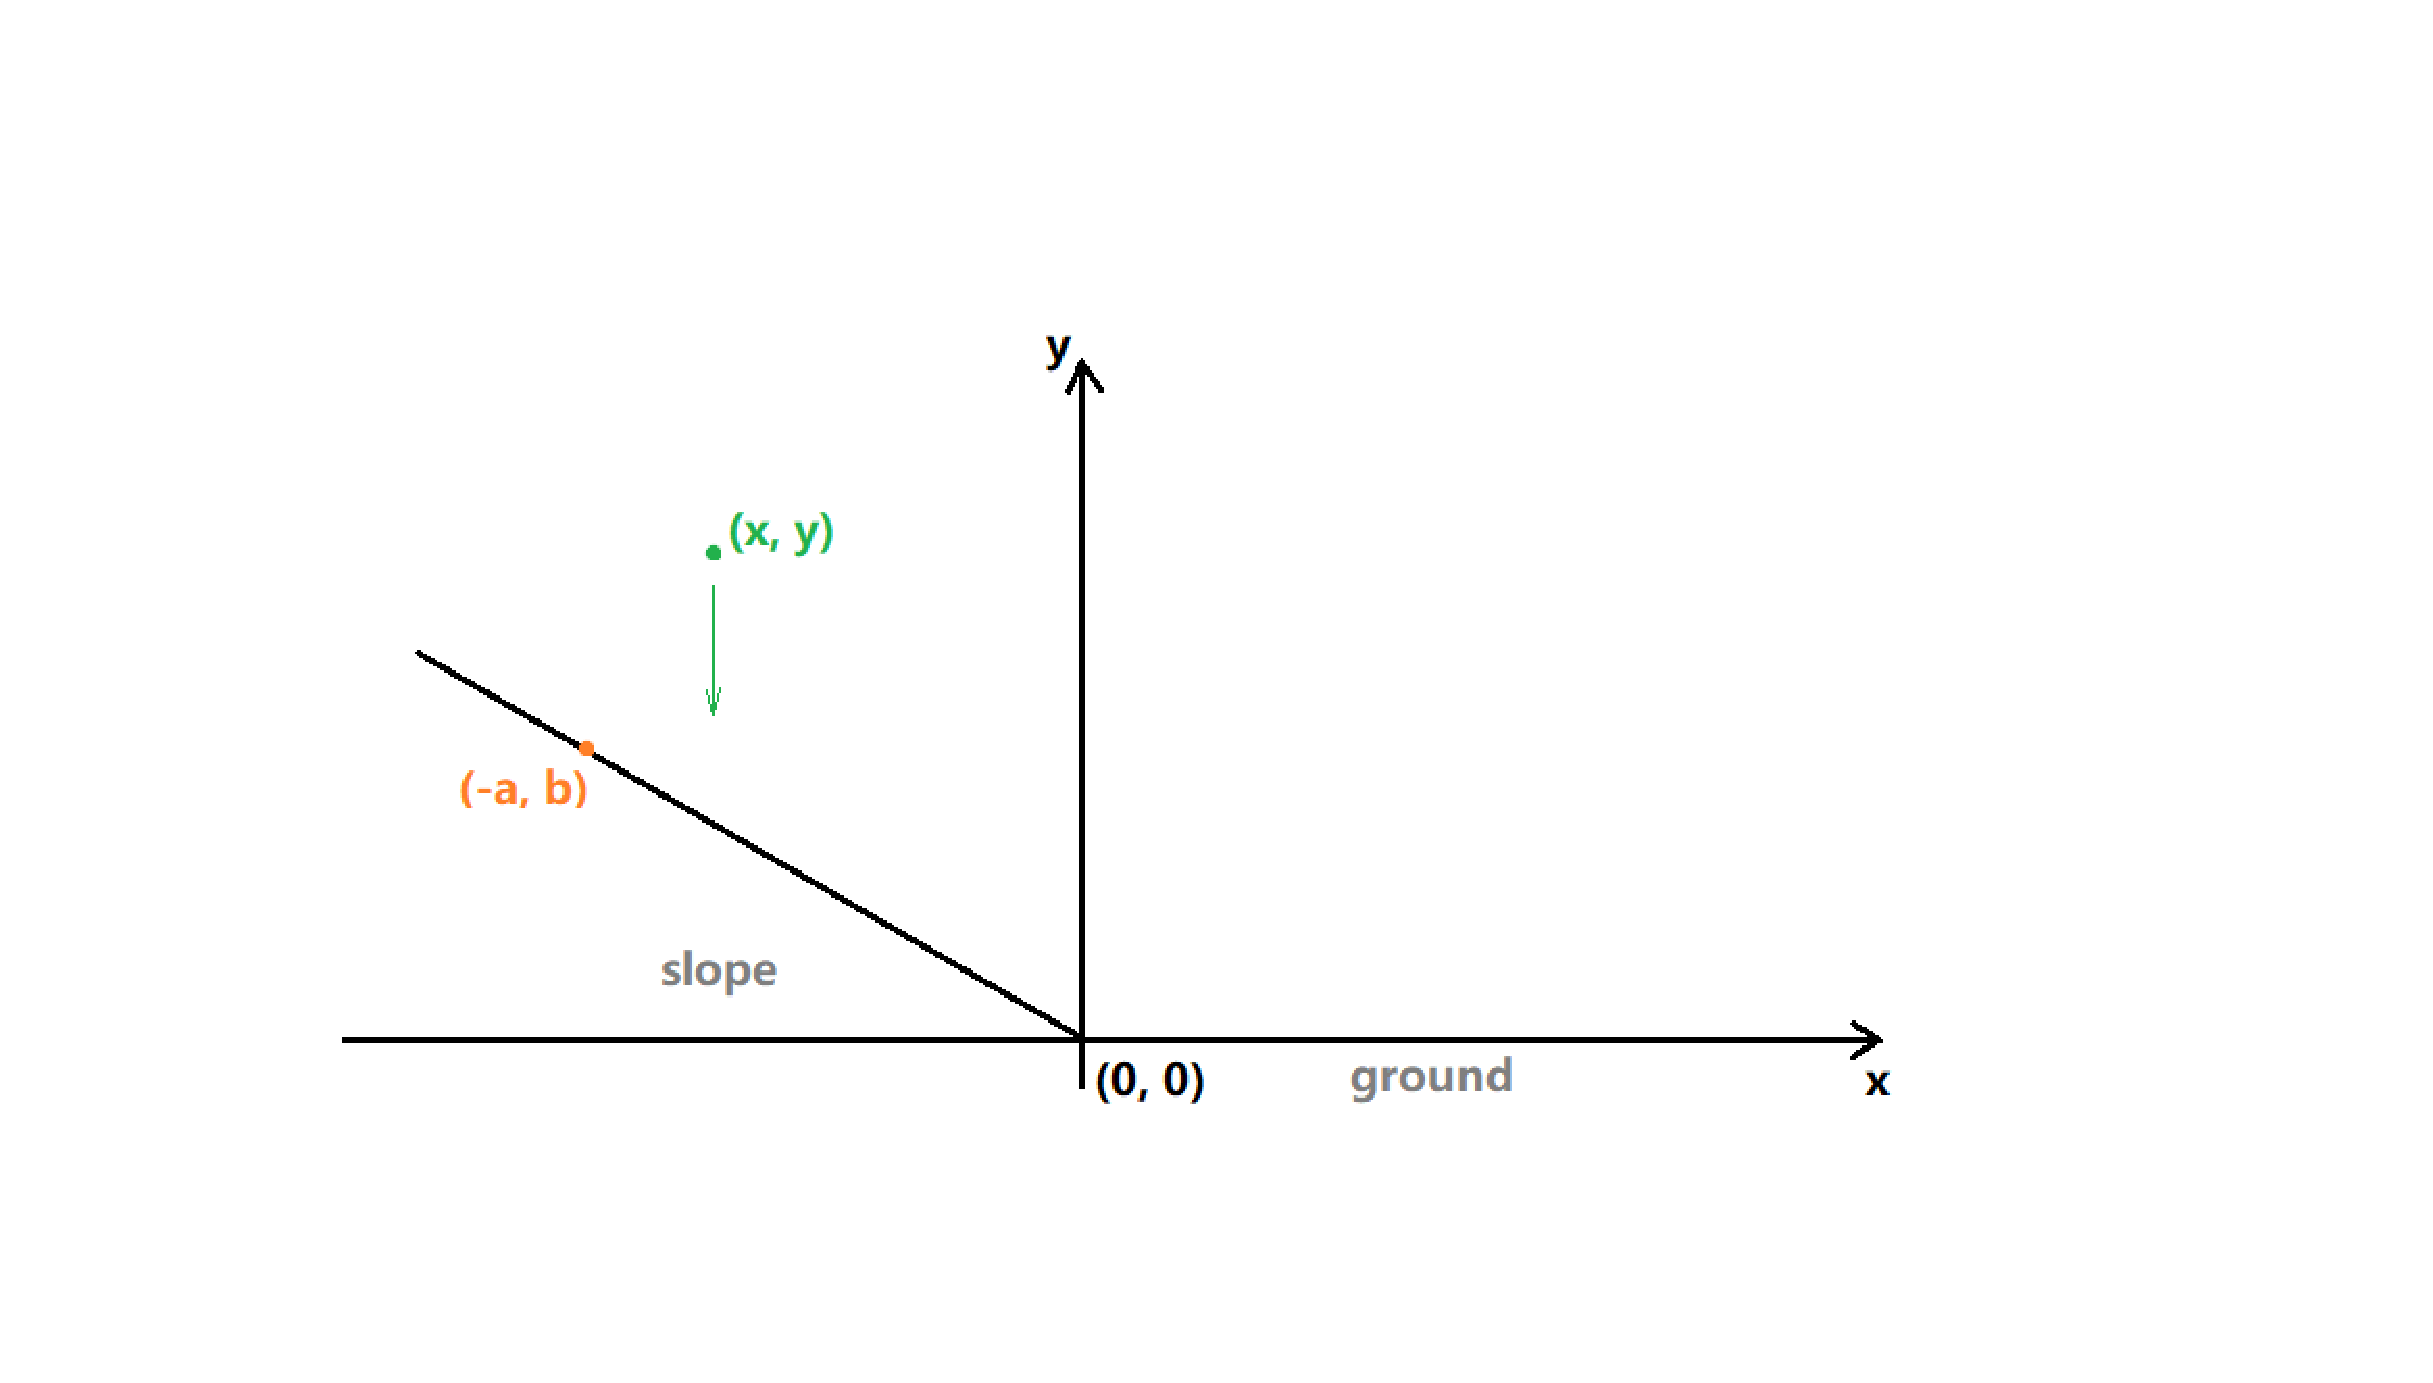
\includegraphics[scale=0.45]{pinball.eps}}

\InputFile
There are multiple test cases. The first line of input contains an integer T (1 $\le$ T $\le$ 100), indicating the number of test cases.

The first line of each test case contains four integers a, b, x, y (1 $\le$ a, b, -x, y $\le$ 100), indicate that the slope will pass through the point(-a, b), the initial position of the ball is (x, y).

\OutputFile
Output the answer.

It's guarantee that the answer will not exceed 50.

\Example

\begin{example}
\exmp{1
5 1 -5 3
}{2
}%
\end{example}

\end{problem}

